\section{控制系统中的传感器}

\subsection{控制系统}

\begin{figure}[H]
	\centering
	\begin{tikzpicture}[node distance=2cm]

	% 节点
	% \node[startstop] (start) {开始};
	% \node[block, below=of start] (step1) {步骤 1};
	% \node[decision, below=of step1] (decide) {条件？};
	% \node[block, below left=2cm and 1.5cm of decide] (step2a) {路径 A};
	% \node[block, below right=2cm and 1.5cm of decide] (step2b) {路径 B};
	% \node[startstop, below=3cm of decide] (end) {结束};
	\node[block] (车速传感器) {车速传感器};
	\node[startstop,below=of 车速传感器] (控制器) {控制器};
	\node[block,right=of 控制器] (排肥阻力传感器) {排肥阻力传感器};
	\node[block,above=of 排肥阻力传感器] (肥箱肥量传感器) {肥箱肥量传感器};
	\node[block,below=of 排肥阻力传感器] (流量传感器) {流量传感器};
	\node[startstop,right=of 排肥阻力传感器] (排肥装置) {排肥装置};
	\node[block,below=of 排肥装置] (超声波换能器) {超声波换能器};

	% 连接
	% \draw[arrow] (start) -- (step1);
	% \draw[arrow] (step1) -- (decide);
	% \draw[arrow] (decide) -- node[left] {是} (step2a);
	% \draw[arrow] (decide) -- node[right] {否} (step2b);
	\draw[arrow] (车速传感器) -- node[fill=white]{前进速度} (控制器);
	\draw[arrow] (肥箱肥量传感器) -- node[fill=white]{肥量} (控制器);
	\draw[arrow] (排肥阻力传感器) -- node[fill=white]{力} (控制器);
	\draw[arrow] (流量传感器) -- node[fill=white]{排肥速度} (控制器);
	\draw[arrow] (控制器) |- node[fill=white]{功率} (超声波换能器);
	\draw[arrow] (超声波换能器) -- (排肥装置);
	\draw[arrow] (排肥装置) -- (肥箱肥量传感器);
	\draw[arrow] (排肥装置) -- (排肥阻力传感器);
	\draw[arrow] (排肥装置) -- (流量传感器);

	% 两路径指向结束
	% \draw[arrow] (step2a) |- (end);
	% \draw[arrow] (step2b) |- (end);

	\end{tikzpicture}
	\caption{控制系统示意图}
	\label{pic:控制系统示意图}
\end{figure}

控制系统的设计如图\ref{pic:控制系统示意图}所示，通过检测排肥速率、排肥阻力、剩余肥量和前进速度来闭环地控制超声波换能器的功率。控制思路类似内燃机的点火提前角控制，让排肥阻力和超声波换能器的功耗始终在一个临界点。

\subsection{控制系统用到的传感器}

\subsubsection{车速传感器}

工程中通常采用检测传动系统某部分零件转速的方法来间接获得车速。常用的转速传感器有两种：基于电磁原理的磁阻式转速传感器和基于广电原理的光电编码器。

\paragraph{磁阻式转速传感器}

磁阻式转速传感器具有灵敏度高、零速检测能力好、抗温度变化能力好和可实现更高精度的优点。但是磁阻式转速传感器对磁路设计要求更高，而且对外磁场干扰更敏感。

\paragraph{光电编码器}

光电编码器优点是精度最高，分辨率可达几万PPR，而且响应快、信号清晰、易处理。它的缺点是对灰尘和油污极其敏感、不能承受强震动环境、成本更高。

由于施肥车工作环境比较恶劣，有灰尘干扰，因此应当选择磁阻式的转速传感器。

\begin{figure}[H]
	\centering
	\begin{minipage}[b]{0.45\textwidth}
		\centering
		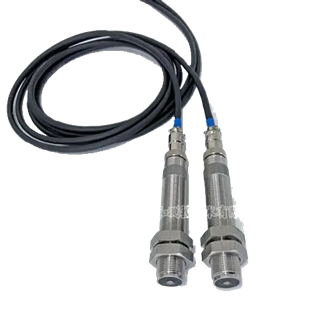
\includegraphics{../../assets/磁阻转速传感器.png}
		\caption{磁阻式转速传感器}
	\end{minipage}
	\begin{minipage}[b]{0.45\textwidth}
		\centering
		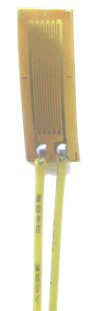
\includegraphics{../../assets/应变片.png}
		\caption{应变片}
	\end{minipage}
\end{figure}

\subsubsection{排肥阻力传感器}

本系统选择使用电阻应变式力传感器（Resistive Strain Gauge Load Cell）来检测排肥阻力。电阻应变式力传感器（电阻应变传感器、应变片力传感器）利用金属材料受力后产生微小变形，贴在其上的应变片电阻随之变化，通过惠斯登电桥转化为电压输出，从而测量力、重量、应变和压力。它是工业上使用最广泛的力传感器类型。

\subsubsection{肥箱肥量传感器}

有机肥属于颗粒材料，而且肥箱是不封顶的，因此许多常见的检测液面高度的传感器都无法使用。同时又由于有机肥会污染传感器，因此需要选择非接触式传感器。综上所述，选择超低频电磁式穿透液位计（外贴式电磁液位检测）。

由于高频磁场会被金属屏蔽，而几十Hz--几kHz的低频磁场能穿透数毫米厚的钢板，所以超低频电磁式穿透液位计的原理是其发射线圈会发射低频磁场并穿透金属，与金属容器内的液体形成磁场损耗，最终由接受线圈检测到变化。由于液体与空气具有不同的电磁特性，因此线圈信号会明显变化，实现液位判断。

由于有机肥含有一定水分，因此该类型传感器也适合用于有机肥在肥箱内的高度检测。

\begin{figure}[H]
	\centering
	\begin{minipage}[t]{0.45\textwidth}
		\centering
		\begin{tikzpicture}
			% \draw[help lines,thin,step=0.2] (0,0) grid (7,6);
			% \draw[help lines,thick,color=red,step=1] (0,0) grid (7,6);
			\begin{scope}
				\clip[decoration={snake}] (0,3) -- (0,0) -- (3,0) -- (3,3) decorate {(3,3) -- (0,3)} -- cycle;
				\shade[top color=blue!10, bottom color=blue!50] (0,0) rectangle (3,4);
			\end{scope}
			\shade[top color=white,bottom color=gray,draw] (3,2.8) rectangle (3.4,3.2);
			\draw[very thick] (0,0) rectangle (3,4);
			\draw[decoration={snake}] decorate {(2.9,3.1) -- (1.9,3.1)};
			\draw[decoration={snake},shift={(0,-0.2)}] decorate {(2.9,3.1) -- (1.9,3.1)};
			\draw[] (3.5,3.1) -- +(1,1.5) node[above]{超低频电磁式穿透液位计};
		\end{tikzpicture}
		\caption{肥箱高度检测示意图}
	\end{minipage}
	\begin{minipage}[t]{0.45\textwidth}
		\centering
		\begin{tikzpicture}
			\begin{scope}
				\clip (0,0) rectangle (4,2);
				\shade[top color=blue!5,bottom color=blue!45] (0,0) rectangle (4,2);
			\end{scope}

			\shade[draw,top color=white,bottom color=gray] (1.6,2) rectangle (2.2,2.4);
			\draw[] (2,2.6) -- +(1,1.5) node[above]{超声波流量传感器};

			\draw[very thick] (0,0) -- (4,0);
			\draw[very thick] (0,2) -- (4,2);

			% \draw[help lines,thin,step=0.2] (0,0) grid (7,6);
			% \draw[help lines,thick,color=red,step=1] (0,0) grid (7,6);
		\end{tikzpicture}
		\caption{排肥流量检测示意图}
	\end{minipage}
\end{figure}

\subsubsection{流量传感器}

由于有机肥散粒体的物理特性，其流动性不如液体，因此许多设置在管内壁的流量传感器会严重影响有机肥的通过性，导致管道堵塞。因此有机肥流量传感器选择非接触式的可以设置在管外的超声波流量传感器。

超声波流量传感器是一种利用超声波在流体中传播速度受流速影响的现象来测量流量的仪表。它以非接触、外夹式安装著称。其特点：不会切断管道、不改变流动、不造成压损。